\begin{itemize}
\item \textbf{State space vs plan space}
\item State space
	\begin{itemize}
	\item Node: state of the world
	\item Plan: path through space
	\end{itemize}
	
\item Plan space
	\begin{itemize}
	\item State: set of partially instantiated operators and some constraints
	\item Impose more constraints until Plan
	\end{itemize}

\item \textbf{Linear search}
\item Work on one goal until completely solved
\item Order of problem solving is linearly-related to order in which plan actions are executed
\item Maintain \textbf{goal stack}
\item Implications
	\begin{itemize}
	\item No interleaving of goal achievement
	\item Efficient search if goals do "not" interact
	\end{itemize}
	
\item \textbf{Means-End analysis}
\item Search relevant aspects of problem, means/operators, ends/goals
	\begin{itemize}
	\item Start from the goal
	\item find difference to start state
	\item find operator that reduces this difference
	\end{itemize}
\item General Problem Solver (GPS)
	
\item \textbf{Forward search}
\\
$s \leftarrow s_0$\\
$\pi \leftarrow empty\_plan$\\
$loop$\\
if s satisfies g $\rightarrow$ return $\pi$\\
$E \leftarrow \{$a ground instance of o $\in$ O, precond(a) true in s\}\\
if $E=\emptyset \rightarrow$ failure\\
nondet choose a $\in$ E\\
$s \leftarrow \gamma(s,a)$\\
$\pi \leftarrow \pi,a$\\
$endloop$
\item = sound,complete
\item breadth-first, best-first
	\begin{itemize}
	\item sound and complete
	\item memory exponential in length of solution
	\end{itemize}
\item depth-first, greedy search
	\begin{itemize}
	\item Worst-case mem is linear in length of solution
	\item Sound, but not complete 
	\item but CP has only finite states $\rightarrow$ loop-checking solves completeness
	\end{itemize}	
\item large branching factor (need good heuristic / pruning)

\item \textbf{Backward search}
\item Means-end analysis
\item start at goal and compute inverse state transitions 
\item a makes at least one of g's literals true and non false
\item $g' = \gamma^{-1}(g,a) = (g\backslash effects(a)) \cup precond(a)$
\\
$\pi \leftarrow empty\_plan$\\
$loop$\\
if s satisfies g $\rightarrow$ return $\pi$\\
$A \leftarrow \{ a|a$ ground instance of o in O and $g' = \gamma^{-1}(g,a)$ defined $\}$\\
if $A=\emptyset$ failure \\
nondet choose $a \in A$ \\
$\pi \leftarrow a,\pi$ \\
$g \leftarrow \gamma^{-1}(g,a)$ \\
$endloop$
\item Branching factor smaller, but can be big because of more actions than needed

\item \textbf{Lifting}
\item reduce branching factor by \textbf{partially instantiating} operators (=lifting)


\item \textbf{STRIPS}
\item STRIPS assumption -> solved frame problem
\item difference
\item sub-goals
\item applicability
\item plan execution and learning

\item \textbf{Block stacking}

%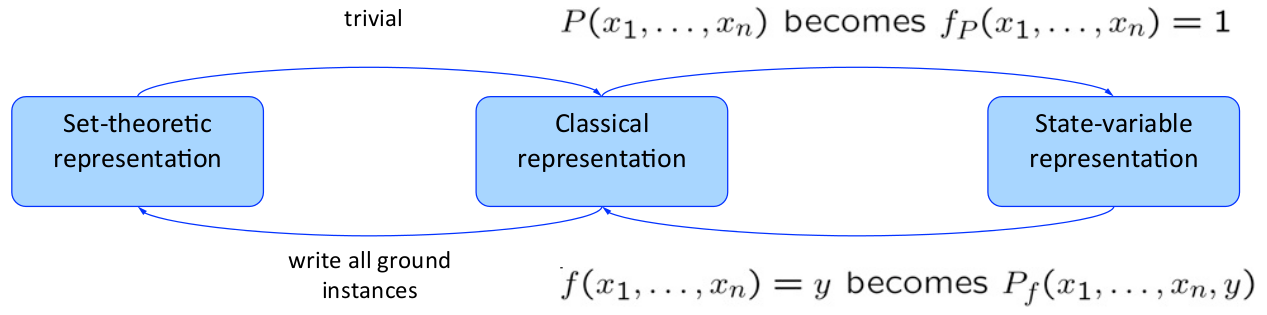
\includegraphics[width=0.48\textwidth]{./img/conversions.png}

\end{itemize}